\subsection{Serverseitige Abweichungen}


\subsection{Implementierte Funktionen des Servers}

\textbf{/FS010/ Benutzerkonten verwalten}

Über \textit{RegistrationRequest} kann man ein neues Benutzerkonto auf dem Server anlegen.\\
Das Benutzerkonto wird an die Geräte-ID des Smartphones gebunden und in der\\
Datenbank des Servers hinterlegt.\\
Mit der \textit{DeleteUserRequest} kann der zuvor erstellte Account gelöscht werden.

\textbf{/FS170/ Umbenennen des Benutzers}

Zusätzlich kann der Benutzer über die \textit{RenameUserRequest} seinen Nutzernamen ändern.

\textbf{/FS030/ Gruppen erstellen / löschen}

Ein registrierter Benutzer kann via \textit{CreateGroupRequest} Gruppen auf dem\\
Server anlegen und per \textit{DeleteGroupRequest} wieder löschen.\\
Der Benutzer ist automatisch in der eigens erstellten Gruppe Admin.

\textbf{/FS040/ Gruppe: Benutzer einladen / entfernen}

Mit der \textit{CreateLinkRequest} kann ein Gruppenadmin einen Einladungslink\\
erstellen. Das im Link enthaltene \textit{'Secret'} wird in der Gruppe auf\\
dem Server hinterlegt.\\
Über die \textit{KickMemberRequest} kann ein Gruppenmitglied aus der Gruppe\\
entfernt werden.

\textbf{/FS180/ Gruppe: Mitglieder zu Administratoren machen}

Mit der \textit{MakeAdminRequest} können Mitglieder zu Admins befördert werden.

\textbf{/FS060/ Gruppe: beitreten / verlassen}

Ein anderer Benutzer kann mit einer \textit{JoinGroupRequest} einer Gruppe beitreten.\\
Das zum Beitreten benutzer \textit{'Secret'} wird aus der Gruppe vom Server gelöscht.\\
Eine Gruppe kann mit der \textit{LeaveGroupRequest} verlassen werden.

\textbf{/FS090/ Gruppe: Treffpunk festlegen}

Mit der \textit{SetAppointmentRequest} kann der Gruppenadmin einen Treffpunkt festlegen.
Dieser wird in der Server-Datenbank gespeichert, wo er von anderen Gruppenmitgliedern
abgerufen werden kann.


\textbf{/FS110/ Gruppe: GPS Daten mitteilen / empfangen}

Per \textit{BroadcastGpsRequest} kann ein Gruppenmitglied der Gruppe seinen Standort
mitteilen. Gleichzeitig erhält er, verpackt in einer \textit{ObjectResponse},
die Standorte der anderen Gruppenmitglieder.

\textbf{/FS190/ Gruppe: Umbenennen}

Analog zur \textit{RenameUserRequest}, kann man mit der \textit{RenameGroupRequest}\\
Den Gruppennamen ändern (der Name muss eindeutig sein).

\textbf{/FS130/ Verschlüsselung}

Transportverschlüsselung wird über HTTPS garantiert.

\subsection{Abweichungen vom Entwurf}

\subsubsection{Request / Response}

Da wird (leider erst nach der Entwurfsphase) festgestellt haben, \\
dass der Jackson ObjectMapper über Annotations auch Polymorphismus unterstützt,\\
ist ein Großteil der Logik in die Requests gewandert.\\
Um uns an das Command-pattern zu halten, haben wir und dazu entschieden, \\
den Requests eine execute() Methode hinzuzufügen. Somit sind Daten und Logik \\
zusammen gekapselt. Das Pattern erschien anfangs hinderlich, da man,\\
sobald sich das Model änderte, alle Requests anpassen musste.\\
Als das Model jedoch fertig war, wurde es sehr einfach, neue Requests für neue\\
Aufgaben hinzuzufügen.\\

Die Response Klassen waren, von Anfang bis Ende, nur Container für Parameter.\\
Zum Vereinfachen haben wir sie zu Response und ObjectResponse zusammengefasst.\\
In einer ObjectResponse können beliebige Objekte die Serializable implementieren,\\
verpackt werden.\\
Das Serializable Interface ist dabei nur für das Abbilden auf Subklassen zuständig,\\
die der ObjectMapper sonst nicht de-serialisieren könnte.\\
Die Requests sind immernoch grob in Group- und User-Requests unterteilt.\\

\subsubsection{Servlets}

Die Umstrukturierungen des Servers, hinsichtlich der Requests, haben dazu gefüht,\\
dass nur noch ein HttpServlet nötig war das MainServlet.\\
Es serialisiert/deserialisiert Request und Response Objekte bearbeitet Http-Anfragen.\\
Die GoApp kommuniziert ausschließlich über POST-Requests mit dem Server.\\
Über eine GET-Anfrage mit beispielsweise einem Webbrowser, \\
erhält man nur die Aufforderung, die App zu installieren.\\

\subsection{Datenbank-Anbindung Server}

\begin{figure}[H]
     \centering
     \hspace*{+0.2cm}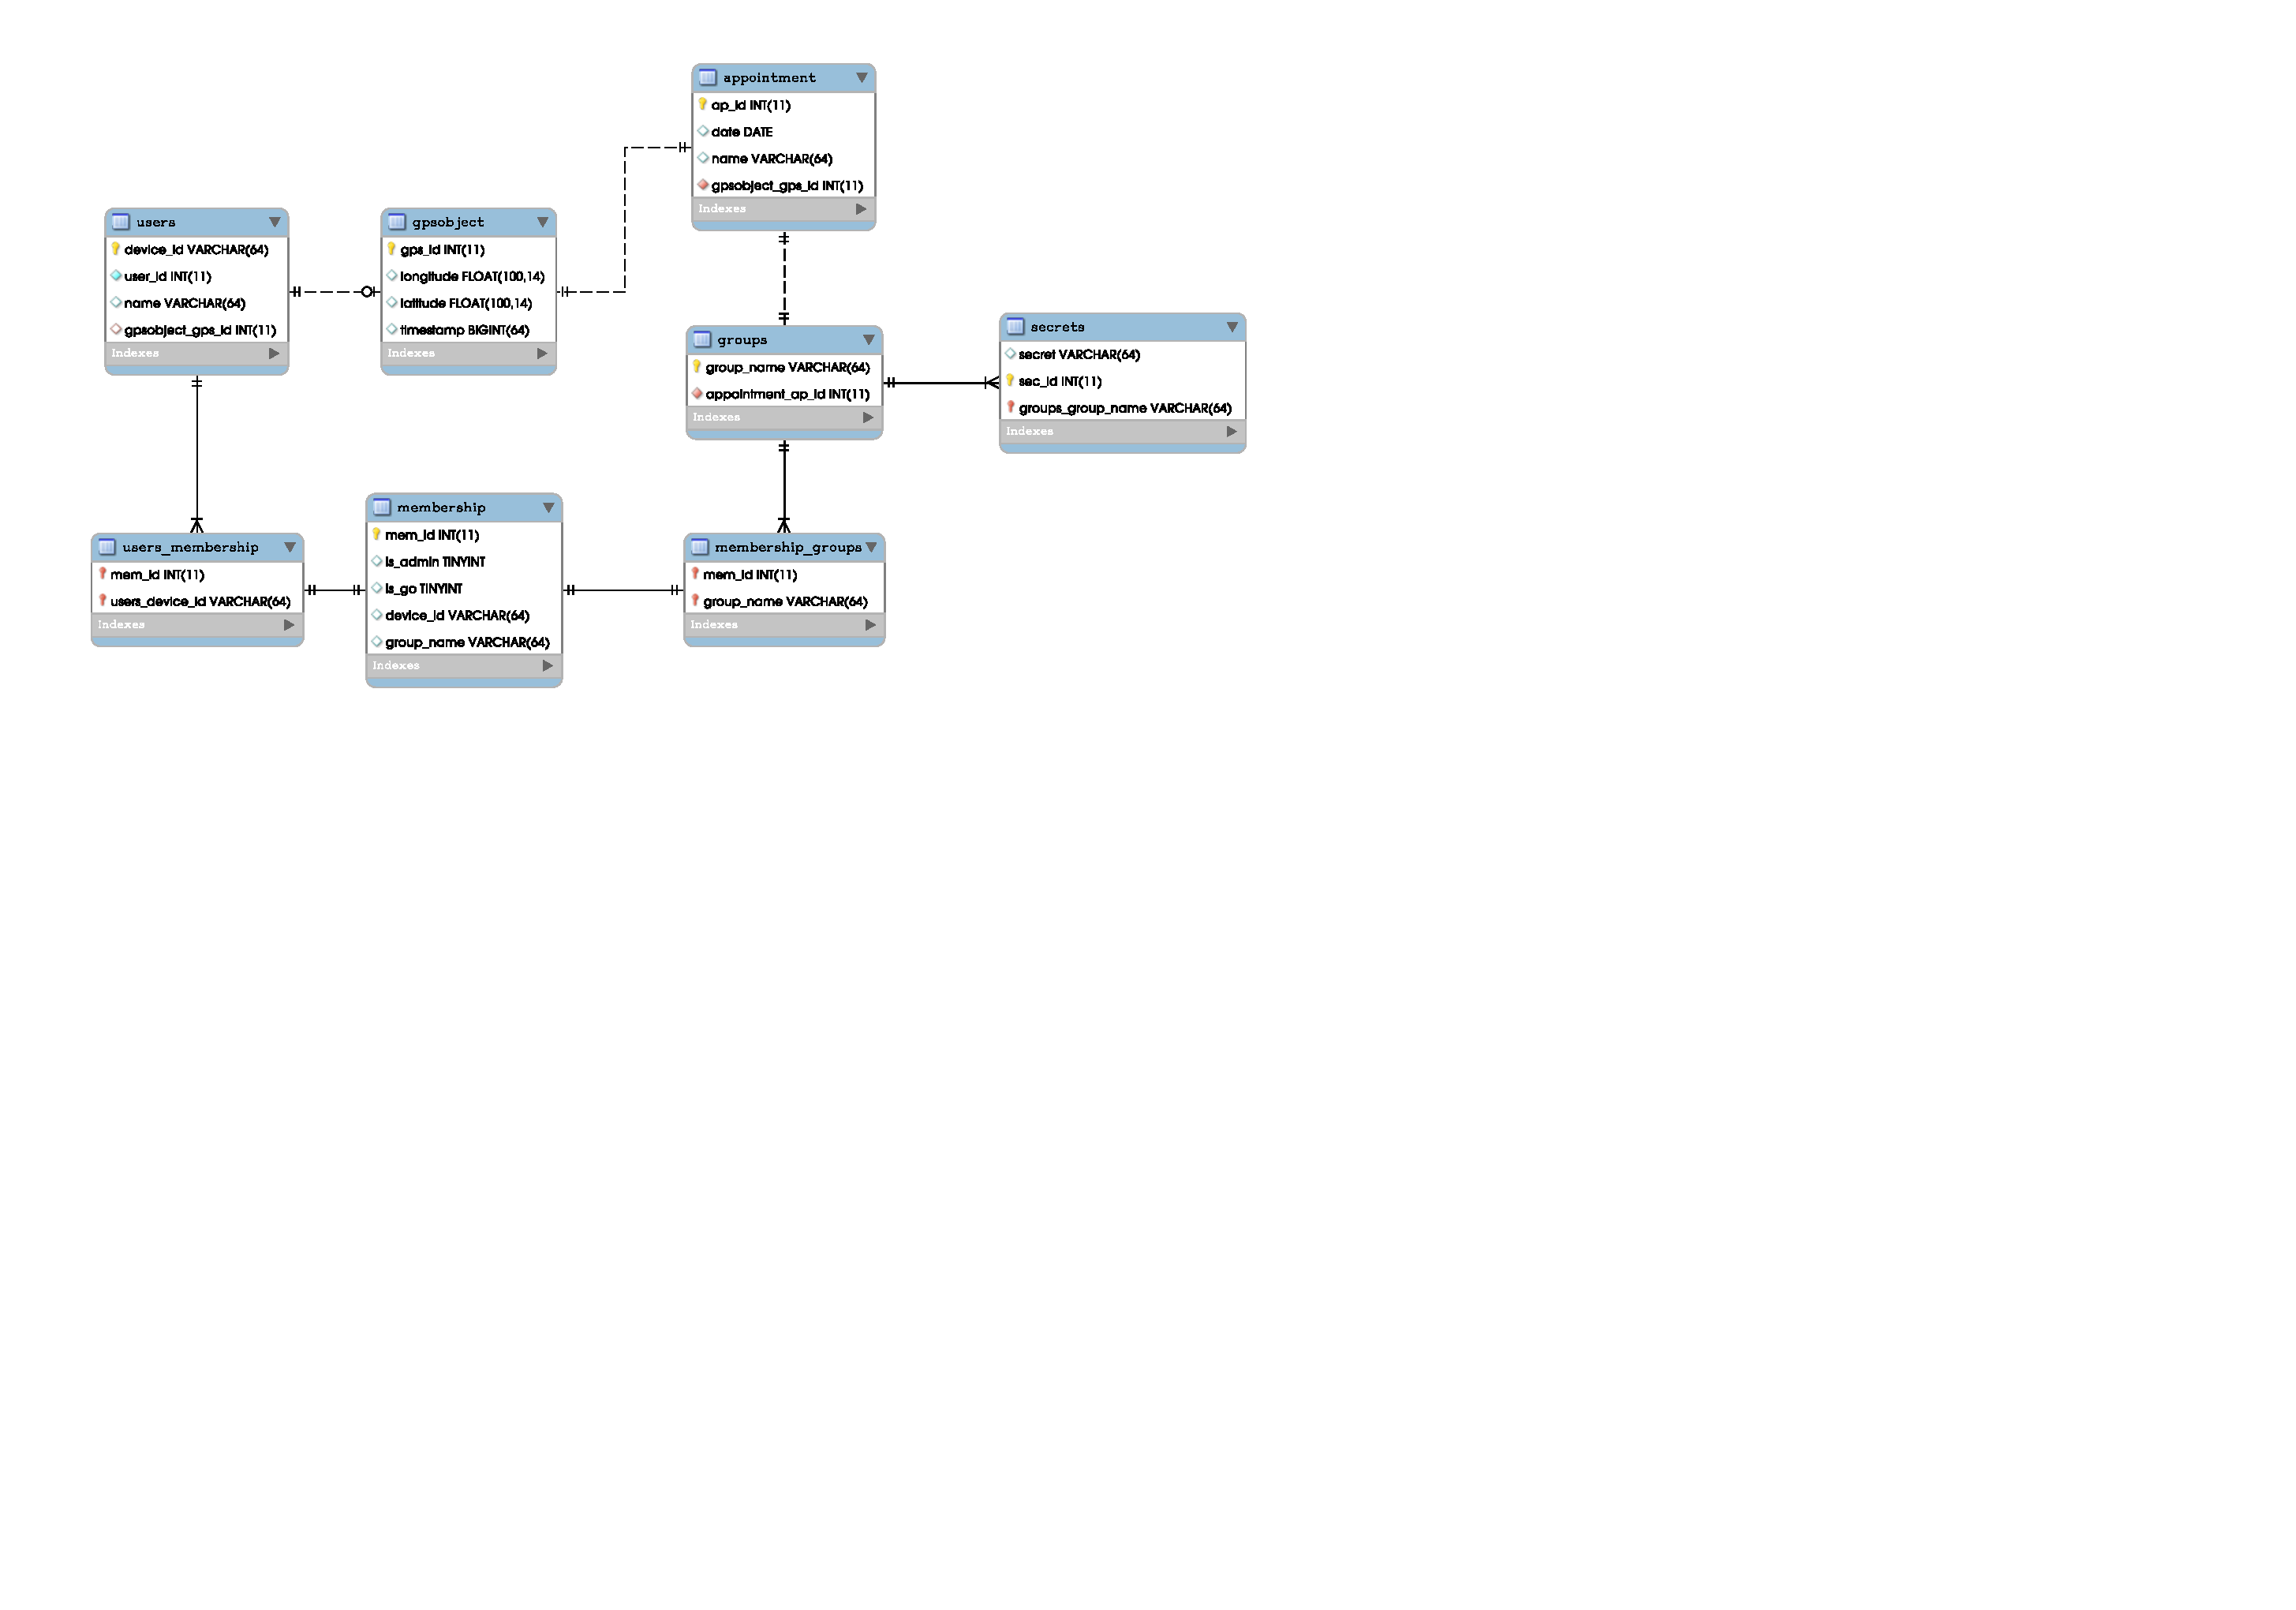
\includegraphics[scale=0.7, trim=125 450 400 30]{db-server}
\end{figure}

Da unser ausgefallenes Gruppenmitglied der Meinung war, dass sich durch die Datenbank\\
nichts an unserem Entwurf ändert, ist es leider auch nicht mit im Entwurf vorhanden.\\
Da das Persistieren einer geschachtelten HashMap nicht ohne weiteres möglich ist,\\
erschien es uns einfacher eine neue Klasse einzuführen, welche die Beziehung zwischen\\
Benutzer und Gruppe modelliert. So entstand eine neue Tabelle Membership\\
und die zugehörige Klasse MemberAssociation. Sie stellt eine ManyToMany Beziehung \\
zwischen Gruppe und Benutzer dar.\\
OneToOne Beziehungen existieren ausserdem zwischen Group und Appointment,\\
Appointment und GpsObject, sowie SimpleUser und GpsObject.\\
Die "Secrets" der Gruppen mussten als Collection ebenfalls in eine neue Tabelle\\
ausgelagert werden.\\

Die Schnittstellen UserManager und GroupManager wurden zu ResourceManager zusammengelegt.\\
Diese zusätzliche Indirektion hat sich als nützlich erwiesen und macht die Datenbank\\
zudem austauschbar.\\

Durch die MemberAssociations wurde auch das UserDecorator-Pattern überflüssig.\\
Darin sind die Attribute gespeichert, die die Beziehung zwischen Benutzer und Gruppe\\
beschreiben (Rechte, Go-Status etc.).\\
